 
\chapter{Nonparametric Hidden Markov Models for Neural Data}

In joint work with Zhe Chen, Matt Johnson, and Matthew Wilson, I have been 
developing nonparametric hierarchical Dirichlet process hidden Markov models 
(HDP-HMMs) for neural spike train recordings and applying them to hippocampal 
data recorded in the Wilson lab. The advantage of these nonparametric methods 
is that the number of states is inferred in a data-driven way, allowing the 
complexity of the model to grow with that of the data. However, inference 
becomes more challenging. In this work, we have conducted a thorough empirical 
study that compares parametric and nonparametric methods, as well as a 
variety of inference algorithms and approaches to setting the hyperparameters 
(which can have a large effect on the subsequent inferences). A preliminary 
version of this work is on the arXiv \cite{linderman2014nonparametric}, and 
we are submitting final revisions to the Journal of Neuroscience Methods 
this week. 

\section{Introduction}

A fundamental goal in neuroscience is to understand how populations of  neurons represent and transmit information about the external world. 
The hippocampus is known to encode information relevant to spatial navigation and episodic memory. 
Spatial representation of the environment is pivotal for navigation in rodents \citep{OKeefe78}.
One type of spatial representation is a topological map, which contains only relative ordering or connectivity information
between spatial locations and is invariant to orientation or deformation. A relevant question of interest is: how can neurons 
downstream of the hippocampus  infer representations of space from 
hippocampal spike  activity without {\em a priori} place field information (namely, without the measurement of spatial correlates)?  
Several reports have been dedicated to the mathematical analysis of this problem \citep{Curto08,Dabaghian12}; however, a data-driven approach 
for analyzing ensemble hippocampal spike data remains missing.  This paper 
employs probabilistic modeling and inference methods to uncover the spatial representation (or topological map) based on the ensemble spike activity. 


Bayesian statistical modeling is a consistent and principled  framework for dealing with uncertainties 
about the observed data \citep{Scott02}.  
The goal of Bayesian inference is to incorporate prior knowledge and constraints
of the problem and to infer the posterior distribution of  unobserved variables of interest \citep{Gelman13}. In recent years, cutting-edge Bayesian methods have become increasingly popular
for data analyses in neuroscience, medicine and biology \citep{Mishchenko11a,Chen11,Chen13,Davidson09,Kloosterman14,Yau11}. Specifically, thanks to ever-growing computing power, Markov chain Monte Carlo (MCMC) methods have been widely used in Bayesian inference. 


In our previous work \citep{Chen12a,Chen14}, we have developed a {\em parametric Bayesian} approach to uncover the neural 
representation of spatial topology embedded in rodent hippocampal population codes during spatial navigation. 
Here we extend the preceding work and consider a {\em nonparametric Bayesian} 
approach. 
The nonparametric Bayesian method brings additional flexibility to the probabilistic model, which allows us 
to model the complex structure of neural data \citep{Teh10,Wood08,Shalchyan14}.  
Specifically, we leverage the so-called a hierarchical Dirichlet process-HMM (HDP-HMM) \citep{Teh06}, which extends the finite-state hidden Markov model (HMM) with a nonparametric, HDP prior and derive corresponding Bayesian inference algorithms. 
We consider both deterministic and stochastic approaches for fully Bayesian inference. 
Based on deterministic approximation, we extend the work of \citep{Chen12a,Johnson14} and use a variational Bayes (VB) method for approximate Bayesian inference.  For MCMC, we adapt the Gibbs sampling approach of \citep{Teh06}, and integrate it with a Hamiltonian  Monte Carlo (HMC) method for hyperparameter inference~\citep{Neal10}. 
To the best of our knowledge, the application of the HDP-HMM to hippocampal ensemble neuronal spike trains and the HMC hyperparameter inference algorithm is novel. 

 
We test the statistical model and inference methods with  both simulation data and experimental data. The latter consists of a recording of rat dorsal hippocampal ensemble spike activity during  open field navigation. Using a decoding analysis and predictive likelihood, we verify and  compare the performance of the proposed Bayesian inference algorithms. We also discuss the results of model selection related to the sample size and the choice of concentration parameter or hyperparameters. Our methods provide an extended tool to analyze rodent hippocampal population codes, which may further empower us to explore important neuroscience questions about neural representation, learning and memory. 
 

\section{Methods: modeling and inference}

\subsection{Basic probabilistic model} 


In our previous work  \citep{Chen12a}, we  used a finite $m$-state HMM to characterize the population spiking activity from a population of $C$ hippocampal place cells. 
It was assumed that first, the animal's spatial location during locomotion, modeled as a latent state process, followed a first-order discrete-state Markov chain $\mathcal{S}=S_{1:T}\equiv \{S_t\}\in\{1,\dots, m\}$, and second, the spike counts of individual place cells at time $t$, conditional on the hidden state $S_t$, followed a Poisson  probability with their respective tuning curve functions ${\bLambda=\{\blambda_c\}=\{\{\lambda_{c,i}\}\}}$. Essentially, we employed a Markov-driven population Poisson firing model with the following probabilistic models 
\begin{align}
p(\by_{1:T}, S_{1:T} \given \bpi, \bP, \bLambda) &= p(\mathcal{S}_1\given \bpi) \prod_{t=2}^T p(S_t \given S_{t-1}, \bP) \prod_{t=1}^T p(\by_t \given S_t, \bLambda),\\
\nonumber p(S_1 \given \bpi) &= \distMultinomial(S_1 \given \bpi), \\
\nonumber p(S_t \given S_{t-1}, \bP) &= \distMultinomial(S_t \given \bP_{S_{t-1},:}), \\
\nonumber p(\by_t \given S_t, \bLambda) &= \prod_{c=1}^C \distPoisson(y_{c,t} \given \lambda_{c,S_t}).
\end{align}
where  $\bP=\{P_{ij}\}$ denotes an $m$-by-$m$ state transition probability matrix, with $P_{ij}$ representing the transition probability from state $i$ to $j$ (since $\sum_{k=1}^m P_{ik}=1$, each row of matrix $\bP$ specifies a multinomial likelihood); $y_{c,t}$ denotes the number of spike counts from the $c$-th cell within the $t$-th temporal bin (here we assume that the rate is defined in the unit bin size of 250 ms) and ${\by}_{1:T}=\{y_{c,t}\}_{C\times T}$ denotes time series of $C$-dimensional  population response vector; and $\distPoisson(y_{c,t}|\lambda_{c,i})$ defines a Poisson distribution with the rate parameter $\lambda_{c,i}$ when $S_t=i$. Finally,  $\log p({\by}_{1:T}|\mathcal{S},\btheta)$ defines the observed data log likelihood given the hidden state sequence $\mathcal{S}$ and all parameters $\btheta=\{\bpi, \bP, \bLambda\}$ (where $\bpi=\{\pi_i\}$ denotes a probability vector for the initial state $S_1$).   

The hidden variables $\mathcal{S}=\{S_{1:T}\}$ are treated as the missing data, ${\by}_{1:T}$ as the observed (incomplete) data, and  their combination $\{S_{1:T},{\by}_{1:T}\}$ as the complete data.

A Bayesian version of this model introduces prior distributions over the parameters. We use the following prior distributions,
\begin{align}
\alpha_0 &\sim \distGamma(a_{\alpha_0}, 1.0) \\
\nonumber \bpi &\sim \distDirichlet(\alpha_0\bone),\\
\nonumber \bP_{i,:} &\sim \distDirichlet(\alpha_0\bone), \\
\nonumber \lambda_{c,i} &\sim \distGamma(a_c^0,b_c^0).
\end{align}
where $\distDirichlet$ denotes the Dirichlet prior distribution, and $\distGamma(a_c^0,b_c^0)$ denotes the gamma prior distribution with 
shape parameter $a_c^0$ and scale parameter $b_c^0$.

\subsection{HDP-HMM}

Model selection is an important issue for statistical modeling and data analysis. 
We have previously proposed a {\em Bayesian deviance information criterion} to select the model size $m$  of HMM \citep{Chen12a,Chen14}. Here we extend the finite-state HMM to an HDP-HMM, a nonparametric Bayesian extension of the HMM that allows for a potentially infinite number of hidden states \citep{Teh06, Beal02}. Namely,  the HDP-HMM treats the priors via a stochastic process. Instead of imposing a Dirichlet prior distribution on the rows of the finite state transition matrix $\bP$, we use a HDP that allows for a countably infinite number of states. 

Specifically, we sample a distribution over latent states,~$G_0$, from a Dirichlet process (DP) \citep{Ferguson73} prior,~${G_0\sim\texttt{DP}(\gamma,H)}$, where~$\gamma$ is the concentration parameter and~$H$ is the base measure. 
Moreover, we place a prior distribution over the concentration parameter,~$\gamma \sim \distGamma(a_{\gamma}, 1.0)$. 
Given the concentration, one may sample from the DP via the ``stick-breaking construction'' \citep{Sethuraman94}. First, sample the stick-breaking weights,~$\bbeta$, 
\begin{eqnarray}                                   
\tilde{\beta}_{i}\sim \texttt{Beta}(1,\gamma), \;\;\; \beta_{i}=\tilde{\beta}_{i}\prod_{j=1}^{i-1}\Big(1-\beta_{j}\Big)
\label{stick1}
\end{eqnarray}
where~$\beta_1 = \tilde{\beta}_1$,~$\sum_{i=1}^\infty \beta_{i}=1$, and $\texttt{Beta}(a,b)$ defines a beta distribution with two positive shape parameters $a$ and $b$. 

The stick-breaking construction of (\ref{stick1}) is sometimes denoted as~${\bbeta \sim \texttt{GEM}(\gamma)}$, after Griffiths, Engen, and McCloskey \citep{Ewens90}. 
The name ``stick-breaking'' comes from the interpretation of $\beta_i$ as the length of the piece of a unit-length stick assigned to the $i$-th value.
After the first $i-1$ values having their portions assigned, the length of the remainder of the stick is broken according  to a sample $\tilde{\pi}_i$
from a beta distribution, and $\tilde{\beta}_i$ indicates the portion of the remainder to be assigned to the $i$-th value. Therefore, the stick-breaking process $\texttt{GEM}(\gamma)$ also defines a DP---the smaller $\gamma$, the less (in a statistical sense) 
of the stick will be left for subsequent values. 

After sampling~$\bbeta$, we next sample the latent state variables, in this case~${\blambda_c}$, from the base measure~$H$. Our draw from the~${\mathrm{DP}(\gamma,H)}$ prior is then given by
\begin{align}
G_0=\sum_{j=1}^\infty \beta_j \delta_{\blambda_{c}^{(j)}}.
\end{align}
Thus, the stick breaking construction makes clear that draws from a Dirichlet process distribution are discrete with probability one.

Given a countably infinite set of shared states, we may then sample the rows of the transition matrix,~${\bP_{i,:}\sim\mathrm{DP}(\alpha_0,\bbeta)}$. We place the same prior over~$\pi$.  The base measure in this case is~$\bbeta$, a countably infinite vector of stick-breaking weights, that serves as the mean of the DP prior over the rows of~$\bP$. The concentration parameter,~$\alpha_0$, governs how concentrated the rows are about the mean. Since the base measure~$\bbeta$ is discrete, each row of~$\bP$ will be able to ``see'' the same set of states. By contrast, if we remove the HDP prior and treat each row of~$P$ as an independent draw from a DP with base measure~$H$, each row would see a disjoint set of states with probability one. In other words, the hierarchical prior is required to provide a discrete (but countably infinite) set of latent states for the HMM.

\subsection{Overdispersed Poisson model}

An interesting consequence of this Bayesian model is that it naturally leads to a distribution of spike counts that is overdispersed relative to simple Poisson model, a feature that has been observed in neural recordings \citep{Goris14}. Recent work has explored the negative binomial (NB) distribution as an alternative to Poisson model, since its two parameters allow for Fano factors greater than one.  The NB distribution can also be seen as a continuous mixture of Poisson distributions (i.e., a compound probability distribution) where the mixing distribution of the Poisson rate is a gamma distribution \citep{Gelman13}. In other words, the NB distribution is viewed as a gamma-Poisson (mixture distribution): 
a $\distPoisson(\lambda)$ distribution whose rate  $\lambda$ is itself a gamma random variable. In our case, the gamma prior over firing rates leads to a negative binomial marginal distribution over~$y_{c,t}$.

Though the marginal spike count at a particular time~$t$ may be marginally distributed according to a negative binomial distribution, it is not necessarily true that a sequence of time bins,~$\by_{1:T}$, will be i.i.d. negative binomials. This arises from the correlations induced by the state transition matrix. Instead,~$\by_{1:T}$ will follow a finite mixture of Poisson distributions, with one component for each latent state. The mixture will be weighted by the marginal probability of the corresponding latent state. However, as the number of visited states grows, and the marginal probability of latent states becomes more uniform, the resulting marginal distribution over the sequence of spike counts inherits the over dispersed nature of the negative binomial distribution. This is particularly true of an HDP-HMM with a high concentration.

 \subsection{Markov chain Monte Carlo (MCMC) inference}


Several MCMC-based inference methods have been developed for the HDP-HMM \citep{Beal02,Teh06,van08}. Some of these previous works use a collapsed Gibbs sampler in which the transition matrix~$P$ and the observation parameters~$\bLambda$ are integrated out \citep{Teh06,van08}. In this work, however, we use a ``weak limit'' approximation in which the DP prior is approximated with a symmetric Dirichlet prior. Specifically, we let
\begin{align}
\label{eq:hdphmm_trans}
\gamma &\sim \distGamma(a_\gamma, 1) \\
\nonumber \alpha_0 &\sim \distGamma(a_{\alpha_0}, 1) \\
\nonumber \bbeta \given \gamma &\sim \distDirichlet(\gamma/M, \ldots, \gamma/M), \\
\nonumber \bpi \given \alpha_0, \bbeta &\sim \distDirichlet(\alpha_0 \beta_1, \ldots, \alpha_0 \beta_M), \\
\nonumber \bP_{i,:} \given \alpha_0, \bbeta &\sim \distDirichlet(\alpha_0 \beta_1, \ldots, \alpha_0 \beta_M).
\end{align}
where $M$ denotes a truncation level for approximating the infinity (which is different from  $m$ in the finite-state setting).
 It can be shown that this prior will weakly converge to the DP prior as the dimensionality of the Dirichlet distribution approaches infinity \citep{Johnson14, Ishwaran02}. With this approximation we can capitalize on forward-backward sampling algorithms to jointly update the latent states~$\mathcal{S}$.  

Previous work has typically been presented with Gaussian or multinomial likelihood models, with the acknowledgement that the same methods work with any exponential family likelihood  when the base measure $H$ is a conjugate prior.
Here we present the Gibbs sampling algorithm of~\citep{Teh06} for the HDP-HMM applied to the special case of independent Poisson observations, and we derive Hamiltonian Monte Carlo (HMC) transitions to sample the cell-specific hyperparameters of the firing rate priors. 

We begin by defining Gibbs updates for the neuronal firing rates~$\bLambda$. Since we are using gamma priors with independent Poisson observations, the model is fully conjugate and simple Gibbs updates suffice. Therefore, we have
\begin{align}
\lambda_{c,i} \given \by, \mathcal{S} &\sim \distGamma\left(\alpha_c^0 + \sum_{t=1}^T y_{c,t} \bbI[S_t=i], \;\beta_c^0 + \sum_{t=1}^T \bbI[S_t=i]\right).
\end{align}

Under the weak limit approximation the priors on~$\bP_{i,:}$ and~$\bpi$ reduce to Dirichlet distributions, which are also conjugate with the finite HMM. Hence we can derive conjugate Gibbs updates for these parameters as well. They take the form:
\begin{align}
\bpi \given \alpha_0, \bbeta &\sim \distDirichlet\left(\alpha_0\bbeta + 1_{S_1}\right),\\
\nonumber \bP_{i,:} \given \alpha_0, \bbeta &\sim \distDirichlet\left(\alpha_0\bbeta + \bn_{i}\right),\\
\nonumber n_{i,j}&=\sum_{t=1}^{T-1} \bbI[S_t=i,S_{t+1}=j],
\end{align}
where~$1_j$ is a unit vector with a one in the~$j$-th entry.

Conditioned upon the firing rates, the initial state distribution, and the transition matrix, we can jointly update the latent states of the HDP-HMM using a {\em  forward filtering, backward sampling} algorithm. Details of this well-known algorithm can be found in \citep{Johnson14b}; the intuition is that in the backward pass of the algorithm, we have a conditional distribution over~$S_t$ given~$S_{t+1:T}$. We can iteratively sample from these distributions as we go backward in time to generate a full sample from~${p(\mathcal{S} \given \bP, \bpi, \bLambda)}$. Jointly sampling these latent states allows us to avoid issues with mixing when individually sampling states that are highly correlated with one another.

Finally, the Dirichlet parameters~$\bbeta$ and the concentration parameters~$\alpha_0$ and~$\gamma$ can be updated as in~\citep{Teh06}. A single iteration of the final algorithm consists of an update for each parameter of the model. The aforementioned updates are based upon previous work; one novel direction that we explore in this work is the sampling of the hyperparameters of the gamma firing rate priors.

\subsubsection{Setting firing rate hyperparameters} 
\label{sec:fr_hypers}
We consider three approaches to setting the hyperparameters of the gamma priors for Poisson firing rates, namely,~${\{\alpha_c^0, \beta_c^0\}}$ for the $c$-th cell.  Note that these parameters are distinct from the parameters of the DP prior. 


\begin{itemize}

\item In the first approach, we estimate these parameters   using an empirical Bayesian (EB) procedure, that is, by maximizing the marginal likelihood of the spike counts. 
For each cell, this may be easily done using standard maximum likelihood estimation for the negative binomial model. 
In practice, we found that without regularization this approach leads to extreme values of the hyperparameters.

 

\item Our second approach samples these hyperparameters using Hamiltonian Monte Carlo (HMC) \citep{Neal10}. We note that for fixed values of the ``shape'' parameter~$\alpha_c^0$, the conditional distribution of the ``scale'' parameter,~$\beta_c^0$ is conjugate with a gamma prior distribution. However, setting the shape parameter \textit{a priori} is challenging because it can have a strong influence on the firing rate distribution. HMC allows us to jointly sample both the shape and the scale parameters simultaneously.

To implement HMC we must have access to both the log probability of the parameters as well as its gradient. Since both parameters are restricted to be positive, we instead reparameterize the problem in terms of their logs. For cell~$c$, the conditional log probability equal to,
\begin{align}
\mathcal{L} &= \log p(\log \alpha_c^0, \log \beta_c^0 \given \bLambda_{c,:}) \\
\nonumber &= \sum_{i=1}^m \log p(\lambda_{c,i} \given \alpha_c^0, \beta_c^0) + \text{const.} \\
\nonumber &= \sum_{i=1}^m \alpha_c^0 \log \beta_c^0 - \log \Gamma(\alpha_c^0) + (\alpha_c^0 - 1) \log \lambda_{c,i} - \beta_c^0 \lambda_{c,i}.
\end{align}
Taking gradients with respect to both parameters yields,
\begin{align}
\frac{\partial \mathcal{L}}{\partial \log \alpha_c^0} &= \sum_{i=1}^m \left[ \log \beta_c^0 -\Psi(\alpha_c^0) + \log \lambda_{c,i} \right] \times \alpha_c^0, \\
\nonumber \frac{\partial \mathcal{L}}{\partial \log \beta_c^0} &= \sum_{i=1}^m \left[ \frac{\alpha_c^0}{\beta_c^0}  - \lambda_{c,i} \right] \times \beta_c^0.
\end{align}
The HMC algorithm uses these gradients to inform a stochastic walk over the posterior distribution. With knowledge of the gradients, HMC can sometimes make large updates to parameters, especially in cases where the parameters are highly correlated under the posterior. 


\item In the final approach, we fix the shape hyperparameter,~$\alpha_c^0$, and infer the scale,~$\beta_c^0$.  We place a gamma prior on the scale,~$\beta_c^0 \sim \distGamma(\mu, \nu)$. Given~$\alpha_c^0$, the conditional distribution of the scale is 
\begin{align}
\beta_c^0 \given \alpha_c^0, \{\lambda_{c,i}\}, \mathcal{S}  &\sim \distGamma\bigg(
\mu + \sum_{i=1}^m \bbI[n_i > 0] \cdot \alpha_c^0, \,
\nu + \sum_{i=1}^m \bbI[n_i > 0] \cdot \lambda_{c,i} \bigg) \\
\nonumber n_i &= \sum_{t=1}^T \bbI[S_t=i].
\end{align}
In the following experiments, we set the shape parameter be~$\alpha_c^0=1$, and we set the scale prior parameters to~$\mu=1$ and~$\nu=1$.  This is equivalent to an exponential prior on rates,~$\lambda_{c,i} \sim \distExponential(\beta_c^0)$, and an exponential prior on the scale~$\beta_c^0 \sim \distExponential(1)$.
One could perform cross validation over the shape parameter, but the exponential prior is a rather weak assumption that enables fully-Bayesian inference.


\end{itemize}


\subsubsection{Predictive log likelihood}
With the parameter and hyperparameter inference complete, we evaluate the performance of our algorithm in terms of its predictive log likelihood on held out test data. We approximate the predictive log likelihood with samples from the posterior distribution generated by our MCMC algorithm. That is,
\begin{align}
\log p(\by_{test} \given \by_{1:T}) &= \log \sum_{\mathcal{S}_{test}} \int_{\bTheta} p\left(\by_{test}, \mathcal{S}_{test} \given \btheta \right) \; p\left(\btheta \given \by_{train} \right) \mathrm{d}\btheta, \\
\nonumber &\approx \log \frac{1}{N} \sum_{n=1}^N \sum_{\mathcal{S}_{test}} p\left(\by_{test},  \mathcal{S}_{test} \given \btheta_n\right),
\end{align}
where~${\btheta=(\bLambda, \bP, \bpi)}$ and~$\{\btheta_n \}_{n=1}^N \sim p(\btheta \given \by_{train})$. The summation over latent state sequences for the test data is performed with the message-passing algorithm for HMMs.

\subsection{Variational Bayes (VB) inference}



We build upon our previous work \citep{Chen12a,Chen14,Johnson14} to develop a variational inference algorithm for fitting the HDP-HMM to hippocampal spike trains. Our objective is to approximate the posterior distribution of the HDP-HMM with a distribution from a more tractable family. As usual, we choose a factorized approximation that allows for tractable optimization of the parameters of the variational model. Specifically, we let,
\begin{align}
p(\mathcal{S}, \bLambda, \bP, \bpi, \bbeta \given \by_{1:T}) &\approx q(\mathcal{S}) q(\bLambda) q(\bP) q(\bpi) q(\bbeta).
\end{align}

Since the independent Poisson observations are conjugate with the gamma firing rate prior distributions, choosing a set of independent gamma distributions for~$q(\bLambda)$ allows for simple variational updates.
\begin{align}
q(\bLambda) &= \prod_{i=1}^M \prod_{c=1}^C \distGamma\left(\tilde{\alpha}_{c,i},\, \tilde{\beta}_{c,i} \right), \\
\nonumber \tilde{\alpha}_{c,i} &\leftarrow \alpha_c^{0} + \sum_{t=1}^T y_{c,t} \mathbb{E}_q\big[\bbI[S_t=i]\big], \\
\nonumber \tilde{\beta}_{c,i} &\leftarrow\beta_c^{0} + \sum_{t=1}^T \mathbb{E}_q\big[\bbI[S_t=i]\big].
\end{align}

Following \citep{Johnson14}, we use a ``direct assignment'' truncation for the HDP \citep{Bryant12, Liang07}. In this scheme, a truncation level~$M$ is chosen {\it a priori} and~$q(\mathcal{S})$ is limited to support only states~${S_t\in\{1,\ldots,M\}}$. The advantage of this approximation is that conjugacy is retained with~$\bLambda$,~$\bP$, and~$\bpi$, and the variational approximation~$q(\mathcal{S})$ reduces to
\begin{align}
q(\mathcal{S}) &= \texttt{HMM}(\tilde{\bP}, \tilde{\bpi}, \tilde{\bLambda}), \\
\nonumber \tilde{\bP} &= \exp\left\{\mathbb{E}_q[\ln \bP]\right\}, \\
\nonumber \tilde{\bpi} &= \exp\left\{\mathbb{E}_q[\ln \bpi]\right\}, \\
\nonumber \tilde{\bLambda} &= \exp\left\{\mathbb{E}_q[\ln p(\by \given \bLambda)]\right\}.
\end{align}
Expectations~${\mathbb{E}_q[S_t=i]}$ can then be computed using standard message-passing algorithms for HMMs.

With the direct assignment truncation, the variational factors for~$\bP_{i,:}$ and~$\bpi$ take on Dirichlet priors. Unlike in the finite-state HMM, however, these Dirichlet priors are now over~${M+1}$ dimensions since the final dimension accounts for all states~${i>M}$. Under the HDP prior we had~${P_{i,:}\sim \texttt{DP}(\alpha_0 \cdot \bbeta)}$, and under the truncation the DP parameter becomes~$\alpha_0 \cdot \bbeta_{1:M+1}$. Again, leveraging the conjugacy of the model, we arrive at the following variational updates:
\begin{align}
q(\bP) &= \prod_{i=1}^M \mathrm{Dir}(\tilde{\balpha}_P^{(i)}), \\
\nonumber (\tilde{\balpha}_P^{(i)})_j &\leftarrow \alpha_0 \beta_j + \mathbb{E}_q[\bbI[S_t=i]\cdot\bbI[S_{t+1}=j]].
\end{align}
We use an analogous update for~$\bpi$.

The principal drawback of the direct assignment truncation is that the prior for~$\bbeta$ is no longer conjugate. This could be avoided with the fully conjugate approach of \citep{Hoffman13}, however, this results in extra bookkeeping and the duplication of states. Instead, following \citep{Johnson14, Bryant12, Liang07}, we use a point estimate for this parameter by setting~${q(\bbeta)=\delta_{\bbeta^*}}$ and use gradient ascent with backtracking line search to update this parameter during inference.

There are a number of hyperparameters to set for the variational approach as well. The hyperparameters~$\alpha_c^0$ and~$\beta_c^0$ of gamma prior on firing rates can be set with empirical Bayes, as above. We resort to cross validation to set the Dirichlet parameter~$\alpha_0$ and the GEM parameter~$\gamma$. 
 

Finally, in order to compute predictive log likelihoods on held out test data, we draw multiple samples~$\{(\bLambda, \mathcal{S}, \bP, \bpi, \bbeta)_n\}_{n=1}^N$ from the variational posterior and approximate the predictive log likelihood as
\begin{align}
\ln p(\by_{test} \given \by_{1:T}) &\approx \ln \mathbb{E}_q\left[p(\by_{test} \given \mathcal{S}, \bLambda,  \bP, \bpi, \bbeta)\right] \\
\nonumber &\approx \ln \frac{1}{N} \sum_{n=1}^N p(\by_{test} \given (\mathcal{S}, \bLambda, \bP, \bpi, \bbeta)_n).
\end{align}

\section{Results}
The inference algorithms were implemented based upon the PyHSMM framework of~\citep{Johnson14b}. The codebase was written in Python with \texttt{C} offloads for the message passing algorithms.  We have extended the codebase to perform hyperparameter inference using the methods described above, and expanded it to tailor to neural spike train analysis. Our code is publicly available ({\url{https://github.com/slinderman/pyhsmm_spiketrains}}).


\begin{figure}
\centering
\begin{subfigure}[t]{5.in}
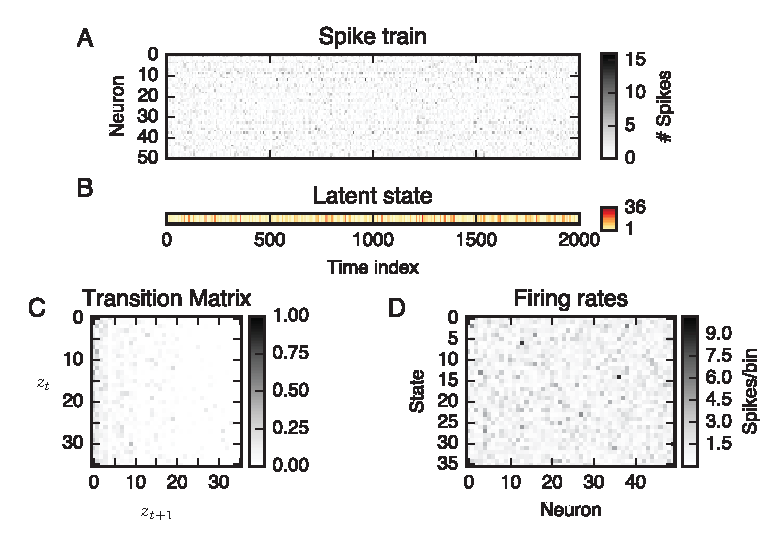
\includegraphics[width=\textwidth]{figures/ch5/Fig1}
\end{subfigure}
\vspace{-.2in}
\caption{An example of a synthetic dataset drawn from an HDP-HMM.  (A) Simulated  population spike trains or spike counts. (B) Inferred latent state sequence. (C) Inferred state transition matrix~$\bP$. (D) Inferred neuronal firing rate vectors~$\blambda_i$ specific to each state.}
\label{fig1}
\end{figure}

 \subsection{Simulation data}

\paragraph{Setup} 
 First, we simulate synthetic spike count data using an HDP-HMM with ${C=50}$ neurons,~${T=2000}$ time bins, and Dirichlet concentration parameters~$\alpha_0=12.0$ and~$\gamma=12.0$. These configuration yield state sequences that tend to visit 30-45 states. All of neuronal firing rate parameters are drawn from a gamma distribution: $\distGamma(\alpha_c^0=1, \beta_c^0=1)$ (with mean 1.0 and standard deviation 1.0). 
 
 An example of one such synthetic dataset is shown in Fig.~\ref{fig1}. The states have been ordered according to their occupancy (i.e., how many times they are visited during the simulation), such that the columns of the transition matrix exhibit a decrease in probability as the incoming state number,~${S}_{t+1}$, increases. This is a characteristic of the HDP-HMM,   indicating the tendency of the model to reuse states with high occupancy.

We compare six combinations of model,  inference algorithm, and hyperparameter selection approaches: (i) HMM with the correct number of states, fit by Gibbs sampling with fixed~$\alpha_c^0=1$; (ii) HMM with the correct number of states, fit by VB with hyperparameters set by empirical Bayes; (iii) HDP-HMM fit by Gibbs sampling with fixed~$\alpha_c^0=1$; (iv) HDP-HMM fit by Gibbs sampling and HMC for hyperparameter updates; (v) HDP-HMM fit by MCMC with hyperparameters set by empirical Bayes; and (vi) HDP-HMM fit by VB with hyperparameters set by empirical Bayes. For the MCMC methods, we set gamma priors over the concentration parameters~($\alpha_0$ and~$\gamma$); for the VB methods, we set~$\alpha_0$ and~$\gamma$ to their true values. Alternatively, they can be selected by cross validation. We set both the weak limit approximation for MCMC and the direct assignment truncation level for VB to~${M=100}$.

We collect 5000 samples from the MCMC algorithms and use the last 2000 for computing predictive log likelihoods. For visualization, we use the final sample to extract the transition matrix and the firing rates. The number of samples and the amount of burn-in iterations were chosen by examining the log probability and parameter traces for convergence. It is found that the MCMC algorithm converges within hundreds of iterations. For further convergence diagnosis of a single Gibbs chain, one may use the autocorrelation tools suggested in \citep{RafteryLewis92,Cowles96}.

We run the VB algorithm for 200 steps to guarantee convergence of the variational lower bound. Again, this is assessed by examining the variational lower bound and is found to converge to a local maxima within tens of iterations.


\paragraph{Assessment} 

We use two criteria for result assessment with simulation data.  The first criterion is based on the Hamming error between the true and inferred state sequences. To compute this, we first relabel the inferred states in order to maximize overlap with the true states. Let~$\mathcal{S}$ be the true state sequence and~$\mathcal{S}'$ be the inferred state sequence. We define the overlap matrix~$O \in \naturals^{M \times M}$ whose entries~$O_{i,j}$ is the number of times the true state is~$i$ and the inferred state is~$j$:
\begin{align}
O_{i,j} &= \sum_{t=1}^T \bbI[S_t=i] \, \bbI[S_t'=j].
\end{align}
We use the Hungarian method~\citep{kuhn1955hungarian} to find a relabeling of the inferred states that maximizes overlap, and then we measure the Hamming error between the true state sequence~$\mathcal{S}$, and the relabeled sequence of inferred states,~$\widetilde{\mathcal{S}}'$:
\begin{align}
\label{eq:hamming}
\text{err}(\mathcal{S}, \widetilde{\mathcal{S}}') &= \sum_{t=1}^T \bbI[S_t \neq \widetilde{S}_t'].
\end{align}

Table~\ref{tab:synth_hamming} summarizes the Hamming error for all six models on five synthetic datasets. We see that the HDP-HMM fit via Gibbs sampling with firing rate hyperparameters set via empirical Bayes outperforms the other models and inference algorithms on three of five datasets, but the HDP-HMM with hyperparameter HMC sampling are very comparable. By contrast, when the models are fit with VB inference, the inferred state sequences tend to use more than the true number of states, which results in very poor Hamming error. Similarly, the HMM fit via Gibbs sampling does not factor in the penalty on additional states and instead tends to use all states equally, resulting in high Hamming error.

\begin{table}
\centering
\caption{Comparison of Hamming error (see Eq.~\ref{eq:hamming})  computed from the same nine simulated data sets as above. The VB inference methods tend to overestimate the number of states and therefore have much higher Hamming error.}
\begin{tabular}{l|ccccc}
Dataset & 1 & 2 & 3 & 4 & 5 \\
\hline
HMM (Gibbs) & 9 & 401 & 13 & 24 & 615 \\
HMM (VB) & 166 & 290 & 295 & 123 & 124 \\
HDP-HMM (Gibbs) & 2 & \bf{3} & 5 & \bf{1} & 6 \\
HDP-HMM (HMC) & 3 & 4 & 3 & 2 & \bf{4} \\
HDP-HMM (EB) & \bf{1} & \bf{3} & \bf{2} & 3 & 12 \\ 
HDP-HMM (VB) & 432 & 586 & 340 & 264 & 675 \\
\hline
\end{tabular}
\label{tab:synth_hamming}
\end{table}

The second criterion is the model's predictive log likelihood (unit: bits/spike) on a held out sequence of~${T_{test}=1000}$ time steps. We compare the predictive log likelihood to that of a set of independent Poisson processes. Their rates and the corresponding predictive log likelihood are given by,
\begin{align}
\widehat{\lambda}_c&=\frac{1}{T_{train}}\sum_{t=1}^{T_{train}} y_{c,t}, \\
\log p(\by_{test} \given \by_{train}) &= \sum_{c=1}^C \left[ -T_{test} \widehat{\lambda}_c + \sum_{t=1}^{T_{test}} y_{c,t} \log \widehat{\lambda}_c  \right].
\end{align}
The improvement obtained by a model is measured in bits, and is normalized by the number of spikes in the test dataset in order to obtain comparable units for each of the test datasets.

Table~\ref{tab:synth_pll} summarizes the predictive log likelihood
comparison.  For all five datasets, the HDP-HMM fit via Gibbs sampling
with fixed~$\alpha_c^0$ performs best, though in general the
increase over fitting the HDP-HMM when using HMC or EB for
hyperparameter selection is small. By contrast, the improvement compared 
to fitting with VB  inference or using a parametric HMM is 
quite significant.

Though computation cost is often a major factor with Bayesian
inference, with the optimized PyHSMM package, the models can be fit to
the synthetic data in under 10 minutes on an Apple MacBook Air. The
runtime necessarily grows the number of neurons and the truncation
limit on the number of latent states. As the model complexity grows,
we must also run our MCMC algorithm for more iterations, which often
motivates the use of variational inference algorithms instead. Given
our optimized implementation and the performance improvements yielded
by MCMC, we opted for a fully-Bayesian approach using MCMC with HMC
for hyperparameter sampling in our subsequent experiments.

\begin{table}
\centering
\caption{Comparison of predictive log likelihood (bits/spike)  computed from 9 simulated data sets, measured in bits per spike improvement over a baseline of independent, homogeneous Poisson processes (the best result in each data set is marked in bold font). }
\begin{tabular}{l|ccccc}
Dataset & 1 & 2 & 3 & 4 & 5 \\
\hline
HMM (Gibbs) & 0.315 & 0.300 & 0.312 & 0.310 & 0.250 \\
HMM (VB)  & 0.298 & 0.290 & 0.313 & 0.306 & 0.252 \\ 
HDP-HMM (Gibbs) & \bf{0.323} & \bf{0.307} & \bf{0.321} & \bf{0.318} & \bf{0.259} \\
HDP-HMM (HMC) & \bf{0.323} & 0.306 & 0.320 & \bf{0.318} & \bf{0.259} \\
HDP-HMM (EB)  & 0.322 & 0.306 & \bf{0.321} & \bf{0.318} & \bf{0.259} \\
HDP-HMM (VB)  & 0.312 & 0.291 & 0.309 & 0.305 & 0.244 \\
\hline
\end{tabular}
\label{tab:synth_pll}
\end{table}

 
\begin{figure}
  \centering
  \begin{subfigure}[t]{5in}
    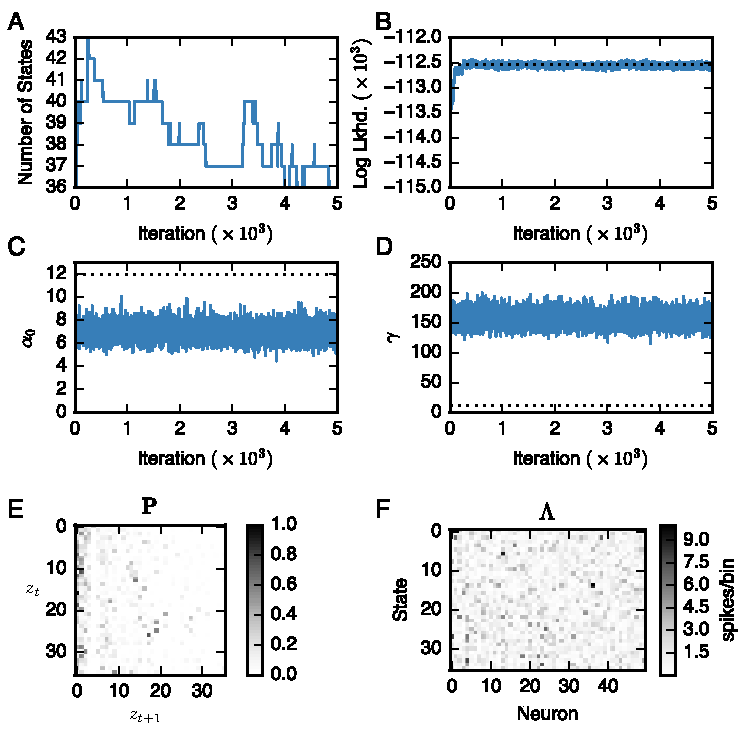
\includegraphics[width=\textwidth]{figures/ch5/Fig2}
  \end{subfigure}
  \caption{MCMC state trajectories for an HDP-HMM fit to the synthetic dataset shown in Fig.~\ref{fig1}. True values are shown by the dotted black lines. The first five iterations of the Markov chain are omitted since they differ greatly from the final states. The chain quickly converges to nearly the correct number of states (A) and achieves close to the true log likelihood (B). (C, D) The chain trajectories of hyperparameters $\alpha_0$ and $\gamma$. (E, F) Inferred state transition matrix and neuronal firing map drawn from the last iteration.  }
  \label{fig2}
\end{figure}

Figure~\ref{fig2} shows example traces from the MCMC combined with HMC algorithm for the HDP-HMM running on synthetic dataset 1. This is the same data from which Fig.~\ref{fig1} is generated. The first 5 Markov chain iterations have been omitted to highlight the variation in the latter samples (the first few iterations rapidly move away from the initial conditions). We see that the log likelihood of the data rapidly converges to nearly that of the true model (horizontal dotted line), and the number of states quickly converges to around~$m=35$.  Note that the nuisance parameters $\alpha_0$  and $\gamma$ do not converge to the true values --- this is due to the fact that the solution is insensitive to these parameters or the presence of local optima.  However, even the concentration parameters are different from the true values,  they are still consistent with the inferred state transition matrix. 

\begin{figure}  
  \centering
  \begin{subfigure}[t]{5in}
    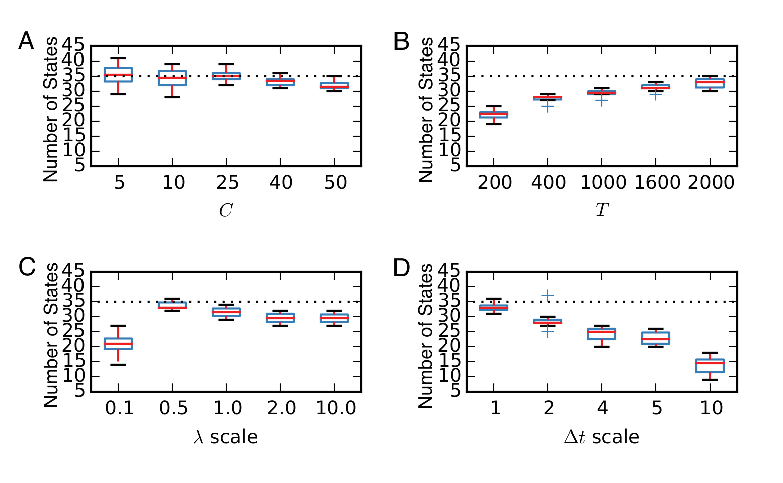
\includegraphics[width=\textwidth]{figures/ch5/Fig3}
  \end{subfigure}
  \caption{In a synthetic data experiment, we generated a spike train for a population of~$C_{\textsf{true}}=50$ cells and~$T_{\textsf{true}}=2000$ time bins. Then we varied the number of observed cells $C$, recording duration $T$, scale of the firing rate $\lambda$, temporal bin size $\Delta t$, and measured the number of inferred latent states. Horizontal dashed lines indicate the ground truth.}
  \label{fig3}
\end{figure}


\paragraph{Sensitivity of the number of latent states} 


To test the sensitivity of the number of inferred states to changes in the data, we vary a number of parameters and plotted the number of inferred states in Fig.~\ref{fig3}. In all cases, we use synthetic dataset~1, shown in Fig.~\ref{fig1}, and HDP-HMMs fit via Gibbs sampling with fixed~$\alpha_c^0$. First, we vary the number of observed cells,~$C$, and find that the number of inferred states was relatively stable around the true number of states ($m=35$). By contrast, as we increase the observed recording length,~$T$, the number of inferred states increases as well. This is because the true underlying data actually does visit more states as we simulate it for longer time. In general, we expect the number of inferred states to grow with the complexity of the data. Next, we vary the scale of the firing rate by multiplying the true model's firing rate by a factor of~$0.1$,~$0.5$, $1.0$, $2.0$, or~$10.0$, and sampling a new spike count. When the rates are very low, most bins do not contain any spikes, and hence it is not possible to resolve as many states. By contrast, when the rate is increased, the number of inferred states is slightly lower than the true number, which is likely the result of a slight mismatch with the prior on the firing rate scale~(parameters~$\mu$ and~$\nu$ in Section~\ref{sec:fr_hypers}). Finally, we considerate the effect of time bin size by scaling up the bin sizes by factors of~$2$ through~$10$. For example, when scaling by a factor of 2, we add the spike counts in each pair of adjacent bins. This has a similar effect to decreasing the recording length by a factor of 2, and hence we see the number of inferred states decrease with bin size.

 \subsection{Rat hippocampal neuronal ensemble data} 

Next, we apply the proposed methods to experimental data of the rat hippocampus. 
Experiments were conducted under the supervision of the Massachusetts Institute of Technology (MIT)  Committee on Animal Care and followed the NIH guidelines.
The micro-drive arrays containing multiple tetrodes were implanted above the  right dorsal hippocampus of male Long-Evans rats. The tetrodes were slowly lowered into the brain reaching the cell layer of CA1 two to four weeks following the date of surgery. Recorded spikes were manually  clustered and sorted to obtain single units using a custom software (XClust, M.A.W.). 


For demonstration purpose, an ensemble spike train recording of~${C=47}$ cells was collected from a single rat for a duration of 9.8 minutes.
Once   stable hippocampal units were obtained, the rat was allowed to freely forage in an approximately circular open field environment (radius: $\sim$60 cm). 
We bin the ensemble spike activity with a bin size of 250 ms and obtain the population vector $\by_t$ in time. 
To identify the period of rodent locomotion during spatial navigation, we use a velocity threshold ($>$10 cm/s) to select the RUN epochs and merge them together. 
One animal's RUN trajectory  and spatial occupancy are shown in Fig.~\ref{fig4} (left and right panels, respectively). The empirical probability of a location,~${p(\ell)}$, is determined by dividing the arena into 220 bins of equal area (11 angular bins and 20 radial bins) and counting the fraction of time points in which the rat is in the corresponding bin. 

\begin{figure}
\centering
\begin{subfigure}[t]{\textwidth}
\centering
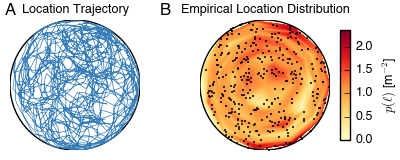
\includegraphics[width=4in]{figures/ch5/Fig4}
\end{subfigure}
\caption{One rat's behavioral trajectory (left) and spatial occupancy (right) in the open field environment. }
\label{fig4}
\end{figure}

In experimental data analysis, we focus on  nonparametric Bayesian inference for HDP-HMM.
For all methods, we increase the truncation level to a large value of $M=100$.  To discover the model order of the variational solutions, we use the number of states visited by the most likely state sequence under the variational posterior. The MCMC algorithms yield samples of state sequences from which the model order can be directly counted. 


\begin{table}
\centering
\caption{A comparison of HMMs, HDP-HMMs, and inference algorithms on the rat hippocampal data. Performance is measured in predictive log likelihood and mean decoding error on two minutes of held out test data (the best result is marked in bold font).} 
\begin{tabular}{l|cc}
& Pred. log likelihood (bits/spike) & Decoding error (cm) \\
\hline 
  HMM ($m=25$)         & 0.712 & $10.85 \pm 6.43$ \\
  HMM ($m=45$)         & 0.706 & $10.71 \pm 6.67$\\
  HMM ($m=65$)         & 0.717 & $11.01 \pm 6.93$\\
  HDP-HMM (Gibbs)    & \bf{0.722} & $\mathbf{9.56 \pm 5.31}$ \\
  HDP-HMM (HMC)      & 0.646 & $9.96 \pm 6.05$\\
  HDP-HMM (EB)       & 0.579 & $10.81 \pm 6.78$\\
  HDP-HMM (VB)       & 0.602 & $10.93 \pm 6.24$\\

 \hline
\end{tabular}
\label{tab:hipp_err}
\end{table}

We perform a quantitative comparison between HMMs, HDP-HMMs, inference algorithms, and hyperparameter setting algorithms, where performance is measured in terms of both decoding error and predictive log likelihood. For both metrics, we train the models on the first $7.8$~minutes of data and test on the final two minutes of data for prediction. The results are summarized in Table~\ref{tab:hipp_err}. We find that the HDP-HMM fit by Gibbs sampling with fixed firing rate scale~($\alpha_c^0=1$) again outperforms the competing models in both measures.

\begin{figure}
\centering
\begin{subfigure}[t]{5in}
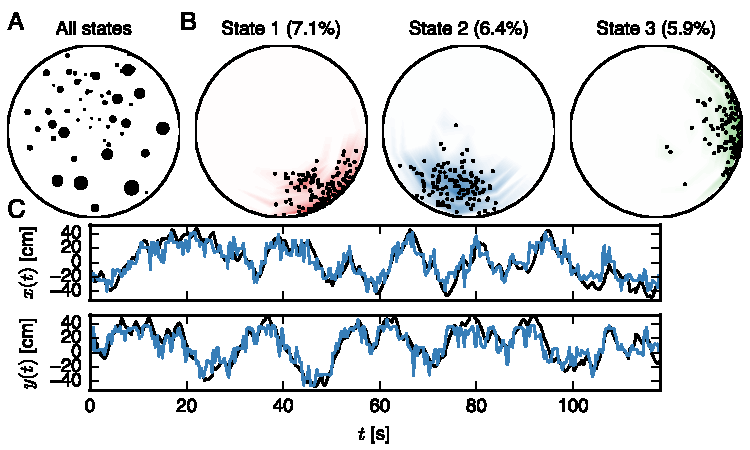
\includegraphics[width=\textwidth]{figures/ch5/Fig5}
\end{subfigure}
\caption{Estimation result from HDP-HMM (Gibbs) for the rat hippocampal ensemble spike data. (A) Estimated state space map, where the mean value of the spatial position for each latent state is shown by a black dot. The size of the dot is proportional to the occupancy of the state.  (B) Probability distributions over location corresponding to the top three latent states, measured by state occupancy. The small black dots indicate the location of the animal while in that state, and are used to compute the empirical distribution over location indicated by colored shading. (C)  The true and reconstructed trajectories in Cartesian coordinate. The true trajectory  is shown in black and the reconstructed trajectory is shown in blue. For each time bin, we use the mean location of the latent states to determine an estimate of the animal's location. }
\label{fig5}
\end{figure}


\begin{figure}
\centering
\begin{subfigure}[t]{5.0in}
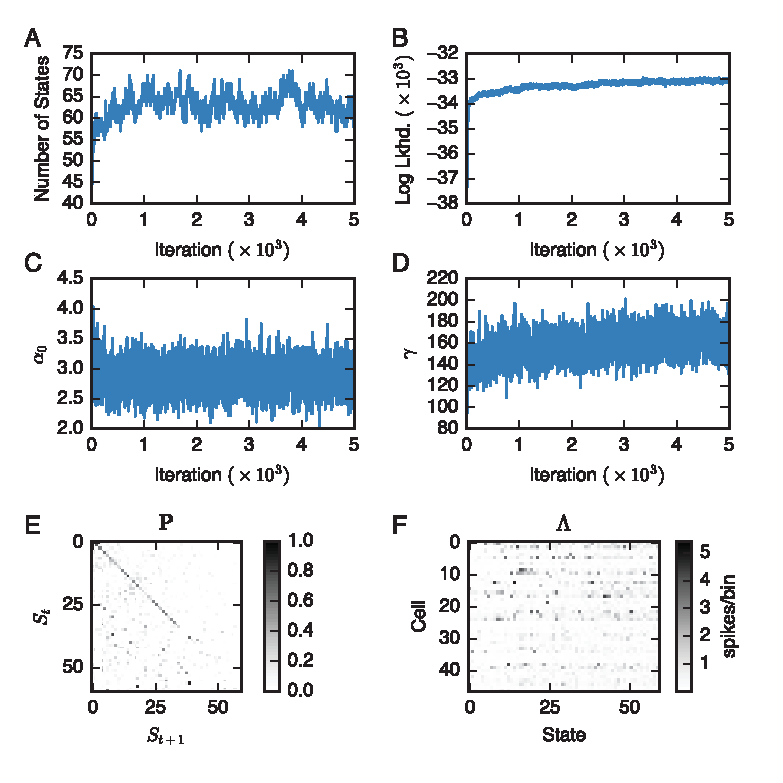
\includegraphics[width=\textwidth]{figures/ch5/Fig6}
\end{subfigure}
\caption{Estimation result from HDP-HMM (Gibbs) for the rat hippocampal ensemble spike data. (A) The total number of states (solid blue) slowly increases as states are allocated for a small number of time bins. The number of states converges after 2500 iterations. (B) The log likelihood of the training data grows consistently as highly specific states are added. (C, D) The concentration parameters,~$\alpha_0$ and~$\gamma$ also converge after 2500 iterations. (E, F) The inferred  state transition matrix and firing rate samples drawn from the last iteration.
}
\label{fig6}
\end{figure}

For the purpose of result assessment, we plot  the state-space or state-location map  (Fig.~\ref{fig5}A), which shows the mean value of the spatial position that each state represented. The size of the black dot is proportional to the occupancy of the state. 
To compute an ``empirical'' distribution over locations for a given state, we first compute the posterior distribution over latent states with our inference algorithms. This gives us a set of probabilities~$\Pr(S_t=i)$ for all time bins~$t$ and states~$i$. Then we compute the average location for each state~$i$ by weighting the animal's location,~$(x_t,y_t)$ by the probability that the animal was in state~$i$ at time~$t$. Summing over time yields a weighted set of locations, which we then bin into equal-area arcs and normalize to get an empirical distribution over locations for each state~$i$. 

The empirical location distribution for the top three states as measured by occupancy are shown in Fig.~\ref{fig5}B). In Fig.~\ref{fig5}C, we show the estimated animal's spatial trajectories in black, along with the reconstructed location in from the HDP-HMM with Gibbs sampling in blue. To reconstruct the position, we use the mean of each latent state's location distribution weighted by the marginal probability of that state under the HDP-HMM. That is,
\begin{align}
\hat{x}_t = \sum_{i=1}^m \bar{x}_i \Pr(\mathcal{S}_t=i), \qquad
\hat{y}_t = \sum_{i=1}^m  \bar{y}_i \Pr(\mathcal{S}_t=i),
\end{align}
where~$\bar{x}_i$ and~$\bar{y}_i$ denote the average location of the rat while in inferred state~$i$ (corresponding to the black dots in Fig.~\ref{fig5}A). Note that the animal's position is not used in model inference, only during result assessment. In the illustrated example (HDP-HMM with MCMC+HMC), the mean reconstruction error in Euclidean distance is 9.07 cm. 



As the parameter sample traces in Fig.~\ref{fig6} show, the Markov chain converges in around 2500 iterations. After this point, the total number of states stabilizes to around~$65$.
The concentration parameters~$\alpha_0$ and~$\gamma$ converge within a similar number of iterations.
Finally, we show the  transition matrix~$\bP$ and firing rate matrix~$\bLambda$ obtained from the final Markov chain  sample.


% Effect of hyperparameters
\begin{figure}
\centering
\begin{subfigure}[t]{5in}
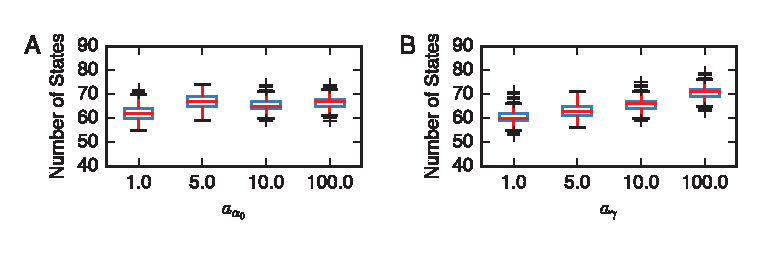
\includegraphics[width=\textwidth]{figures/ch5/Fig7}
\end{subfigure}
\caption{ Measuring the effect of concentration  hyperparameters on the number of inferred latent states. We find that the concentration  hyperparameters of the gamma priors on the concentration parameters,~$\alpha_0$ and~$\gamma$, have a minimal effect.}
\label{fig7}
\end{figure}



We again evaluated the sensitivity of these model fits to the choice of hyperparameters. For the HDP-HMM fit via Gibbs sampling with fixed~$\alpha_c^0$, the primary hyperparameters of interest are the concentration hyperparameters,~$a_{\alpha_0}$ and~$a_{\gamma}$ in Eq.~\ref{eq:hdphmm_trans}, where we have assumed $ \alpha_0 \sim \distGamma(a_{\alpha_0}, 1)$ and $ \gamma \sim \distGamma(a_\gamma, 1) $. 
Figure~\ref{fig7} shows the inferred number of states as we vary these two hyperparameters over orders of magnitude. We found that the number of inferred states is stable around~$65$, indicating the performance robustness to the choice of these hyperparameters. 

% True and inferred place fields
\begin{figure}
\centering
\begin{subfigure}[t]{5in}
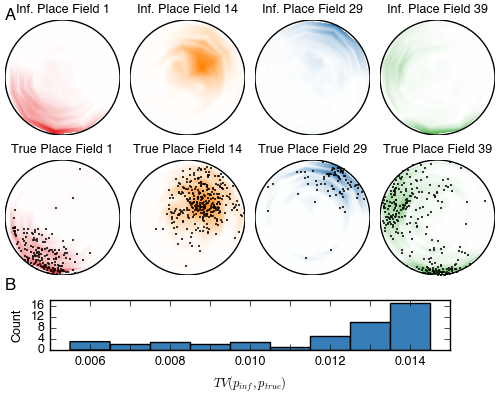
\includegraphics[width=\textwidth]{figures/ch5/Fig8}
\end{subfigure}
\caption{Comparison of inferred and true place fields for four randomly selected hippocampal neurons. The inferred place field (top row) for cell~$c$ is a combination of location distributions for each state~$i$ weighted by the inferred firing rates~$\lambda_{c,i}$, whereas the true place field (bottom row) for cell~$c$ is a histogram of locations in which cell~$c$ fires. The black dots show the rat's locations used for each histogram. The inferred place fields closely match the true place fields. With adequate spike data recording, we expect a higher latent state dimensionality to yield higher spatial resolution in the inferred place fields.}
\label{fig8}
\end{figure}

Looking into the inferred states, we can reconstruct the ``place fields'' or ``state fields'' of hippocampal neurons. To do so, we combine the state-location maps (Fig.~\ref{fig5}B) with the firing rate of the individual neuron  in those states (Fig.~\ref{fig6}F) and weight by the marginal probability of the latent state. Together, these give rise to the inferred neuron's place field. Note that, again, the position data was only used in reconstruction but not in the inference procedure. Four pairs of inferred and true place fields are shown in Fig.~\ref{fig8}. On the top row is the inferred place field; on the bottom is the true place field computed using the locations of the rat when cell~$c$ fired shown by black dots.

% Mutual Info
\begin{figure}
\centering
\begin{subfigure}[t]{2.4in}
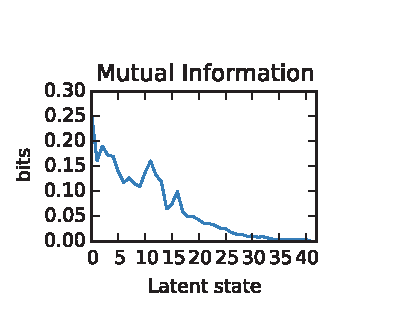
\includegraphics[width=\textwidth]{figures/ch5/Fig9}
\end{subfigure}
\caption{Mutual information of the inferred states and the rat's position. Latent state are ordered by their occupancy, i.e. the number of times the rat was in that state.  }
\label{fig9}
\end{figure}

In addition, we can evaluate the model in terms of the information latent states convey about the rat's position in the circular environment. To do so, we divide the environment into 121 bins of equal area and treat the rat's position as a discrete random variable. Likewise, we treat the latent state as a discrete random variable, and we compute the discrete mutual information between these two variables. 
We  investigate the information content of each individual state by constructing a binary random variable indicating whether or not the model is in state~$i$ and measuring its mutual information with the rat's position. The result is shown in Fig.~\ref{fig9}, where the latent states are ordered in decreasing order of occupancy. As expected, states that are more frequently occupied  carry more information about the rat's position.




\section{Extensions and discussion}

\subsection{Hidden semi-Markovian models}
A striking feature of the inferred state transition matrix in Fig.~\ref{fig6}E is that the first 40 states exhibit strong self-transitions. This is a common feature of time series and has been addressed by a number of augmented Markovian models. In particular, hidden semi-Markovian models (HSMMs) explicitly model the duration of time spent in each state separately from the rest of the state transition matrix \citep{Johnson13}. Building this into the model allows the Dirichlet or HDP prior over state transition vectors to explain the rest of the transitions, which are often more similar. Alternatively, ``sticky'' HMMs and HDP-HMMs accomplish a similar effect \citep{Fox08}.  

\subsection{Statistical and computational considerations}  We have seen a great advantage in nonparametric Bayesian formalism (i.e., HDP-HMM vs. HMM) regarding automatic model selection. This is especially important for sparse sample size or short recording in some neuroscience applications, where cross validation on data is  infeasible.  

For any statistical estimation, we need to consider the ``bias vs. variance'' problem.  
In VB inference, there is a potential estimate bias due to bound optimization (since we optimize the lower bound of the marginal likelihood). In addition, because of the mean-field approximation, the parameter's variance tends to be underestimated. In MCMC inference, the estimate  is asymptotically unbiased, however, if the Markov chain mixes slowly, the estimate's variance can be inaccurate. 

Computationally, the fully-Bayesian HDP-HMM inference is the most demanding. In practice, one can choose various inference tools with gradually increased computational resources (VB, empirical Bayes, Gibbs sampling or HMC) depending on the data sample size and complexity. In addition, the convergence of these algorithm may vary according to the choice of hyperparameters. 


\subsection{Latent state dimensionality and continuous latent state}

In experimental data analysis, the number of identified  states from HDP-HMM depends on  the data as well as the priors of hyperparameters. Given the same size of environment, different numbers of cells or different recording duration  may yield different estimation results (Fig.~\ref{fig3}), since the nonparametric prior allocates states in accordance with the complexity of the data. We found that the weak priors over the concentration parameters have a minimal effect on the number of inferred states (Fig.~\ref{fig7}). Fixing the scale hyperparameter of the firing rate prior distribution and performing Gibbs sampling over the scale of the prior is a simple and robust method. 


 
In our problem, we formulate the latent state is discrete (finite or infinite) and infer the state-transition matrix, from which we can derive the ``topology graph'' of the unknown environment \citep{Chen12a,Chen14}. In parallel to the discrete-state HMM or HDP-HMM, we can also formulate a continuous state-space model, where the state is Gaussian and the observation is Poisson \citep{Brown98,Smith03,Yu09,Buesing12}. Various inference algorithms (Gaussian or variational approximation) have been developed for such models in the literature. Different from discrete state, the continuous-state has a smoother representation (due to infinite spatial resolution). However, similar to the HMM, we will need to deal with the model selection (dimensionality of latent state) problem, which is often tackled by cross validation \citep{Yu09}. In addition, continuous latent state is subject to sign/scale ambiguity. For the purpose of representing space and spatial topology, the discrete-state representation is more appropriate. Provided that the animal's behavior (spatial location) is available, the continuous representation of space will be more accurate. In general, nonparametric Bayesian inference can be applied to continuous or discrete states, as well as continuous or discrete observations \citep{Teh06,van08,Fox08,Fox10,Chen15Book}.



\subsection{Robustness of the population firing model}

A key assumption in our probabilistic model is the Poisson likelihood. Although this assumption may not be true in experimental data, our results have showed excellent performance.   
To further assess the robustness of HDP-HMM-Poisson model in experimental data analysis,
at every  temporal bin we  further add additional  homogeneous non-Poissonian noise  to the observed population spike counts by drawing from a NB distribution (with varying levels of mean 0.25-1.0 and variance 0.5-2.0), and repeat the decoding error analysis. We have found that, as a general trend,  the median decoding error gradually grows as increasing noise mean or variance; yet the decoding performance remains quite satisfactory (results not shown). 



\subsection{Use of soft-labeled spikes}


Thus far, we have assumed that all recorded ensemble spikes are sorted and clustered into single units. Nevertheless, it is known that spike sorting is complex, time-consuming and error-prone \citep{Wood08,Shalchyan14}.
On the one hand,  sorting error is inevitable when there are   overlapping features (such as spike energy, amplitudes or principal components).
On the other hand,  traditional spike-sorting procedures often throw away considerable non-clusterable ``noisy'' spikes, which might contain informative tuning information. How to use these noisy spikes and maximize the information efficiency remains an open question. 
In other words, can we conduct the ensemble spike analysis using unsorted spikes?


Motivated from a sorting-free ensemble decoding analysis \citep{Chen12b,Kloosterman14}, we may use a soft-clustering method based on a Gaussian mixtures model (parameterized by an augmented   vector $\bxi=\{\ell_c,\bmu_c,\bSigma_c\}_{c=1}^K$  that characterizes the weights, mean, and covariance parameters of the Gaussian mixtures). By clustering the spike waveform feature space, we assign each spike with a ``soft'' class label (about the unit identity) according to the posterior probability within the $K$-mixtures. In the feature space, the points close to (far away from) the $c$-th cluster center are associated with a probability assignment value close to (smaller than) 1 in the $c$-th class. Because of the soft membership of individual spikes, the spike count $y_{c,t}$ ($c = 1,\dots, K$) within a time interval can be a non-integer value. Consequently, we replace the variable $C$ with $K$ to indicate that the number of neurons is unknown, and rewrite the  log likelihood as follows   
\begin{eqnarray}                                   
\log p({\by}_{1:T}|\mathcal{S},\btheta,\bxi)= \sum_{t=1}^T \sum_{c=1}^K \log p(y_{c,t}|S_t,\btheta,\bxi)
\end{eqnarray}

In this case, the inference procedure consists of two steps. At the first stage, the $d$-dimensional spike waveform features are clustered 
using a ``constrained'' Gaussian mixture model \citep{Zou12}, which can be either finite or infinite. In the case of infinite Gaussian mixtures, we can also resort to the nonparametric Bayesian approach \citep{Rasmussen99,Gorur10,Wood08}. Upon completing the inference, each spike will be given a posterior probability of being assigned to each cluster. 
At the second stage, we sum the soft-labeled spikes  to obtain the probabilistic spike count $y_{c,t}$ for all $K$-clusters, and the  remaining 
nonparametric Bayesian (MCMC or VB) inference  procedure remains unchanged. A detailed investigation of this idea will be pursued in future work. 




\section{Conclusion}

In this paper, we have explored the use of HDP-HMMs with Poisson likelihoods to analyze rat hippocampal ensemble spike data during spatial navigation. Compared to 
the parametric finite-state HMM, the HDP-HMM allows more flexibility to model the experimental data (without relying on time-consuming cross-validation in model selection). We evaluate two nonparametric Bayesian inference algorithms for HDP-HMM,  one based on VB and the other based on MCMC. Furthermore, we consider two approaches for hyperparameter selection, an issue that is particularly important for the real-life application.  It is found that the MCMC algorithm with HMC updates for the hyperparameters is  robust and achieves the best performance in all simulated and experimental data. Our investigation shows a promising direction in applying nonparametric Bayesian methods for ensemble neuronal spike data analysis.  

The unsupervised Bayesian inference approach  allows us (or hippocampus downstream structures) to read out spatial information from hippocampal ensemble spike activity without {\em a priori} receptive field measurement.
One important future research direction is to apply this method to investigate sleep-associated hippocampal ensemble spike activity  during either slow wave sleep (SWS) or rapid eye movement (REM) sleep \citep{Louie01,Lee02}. Traditionally, one would rely on the place receptive field information estimated from pre-sleep behavior to infer the content of population spike activity in  sleep, but this approach is accompanied with many well-known statistical challenges, such as non-stationarity, firing rate remapping, and timescale warping. Our approach proposed here can provide an effective and complementary paradigm to investigate the representation of hippocampal population codes without direct measurement of spatial correlate \citep{Chen15}. The same principle can also be applied to neocortical data \citep{Ji07,Peyrache09,Gulati14}.  


